\begin{figure}[tbh]
    \begin{center}
        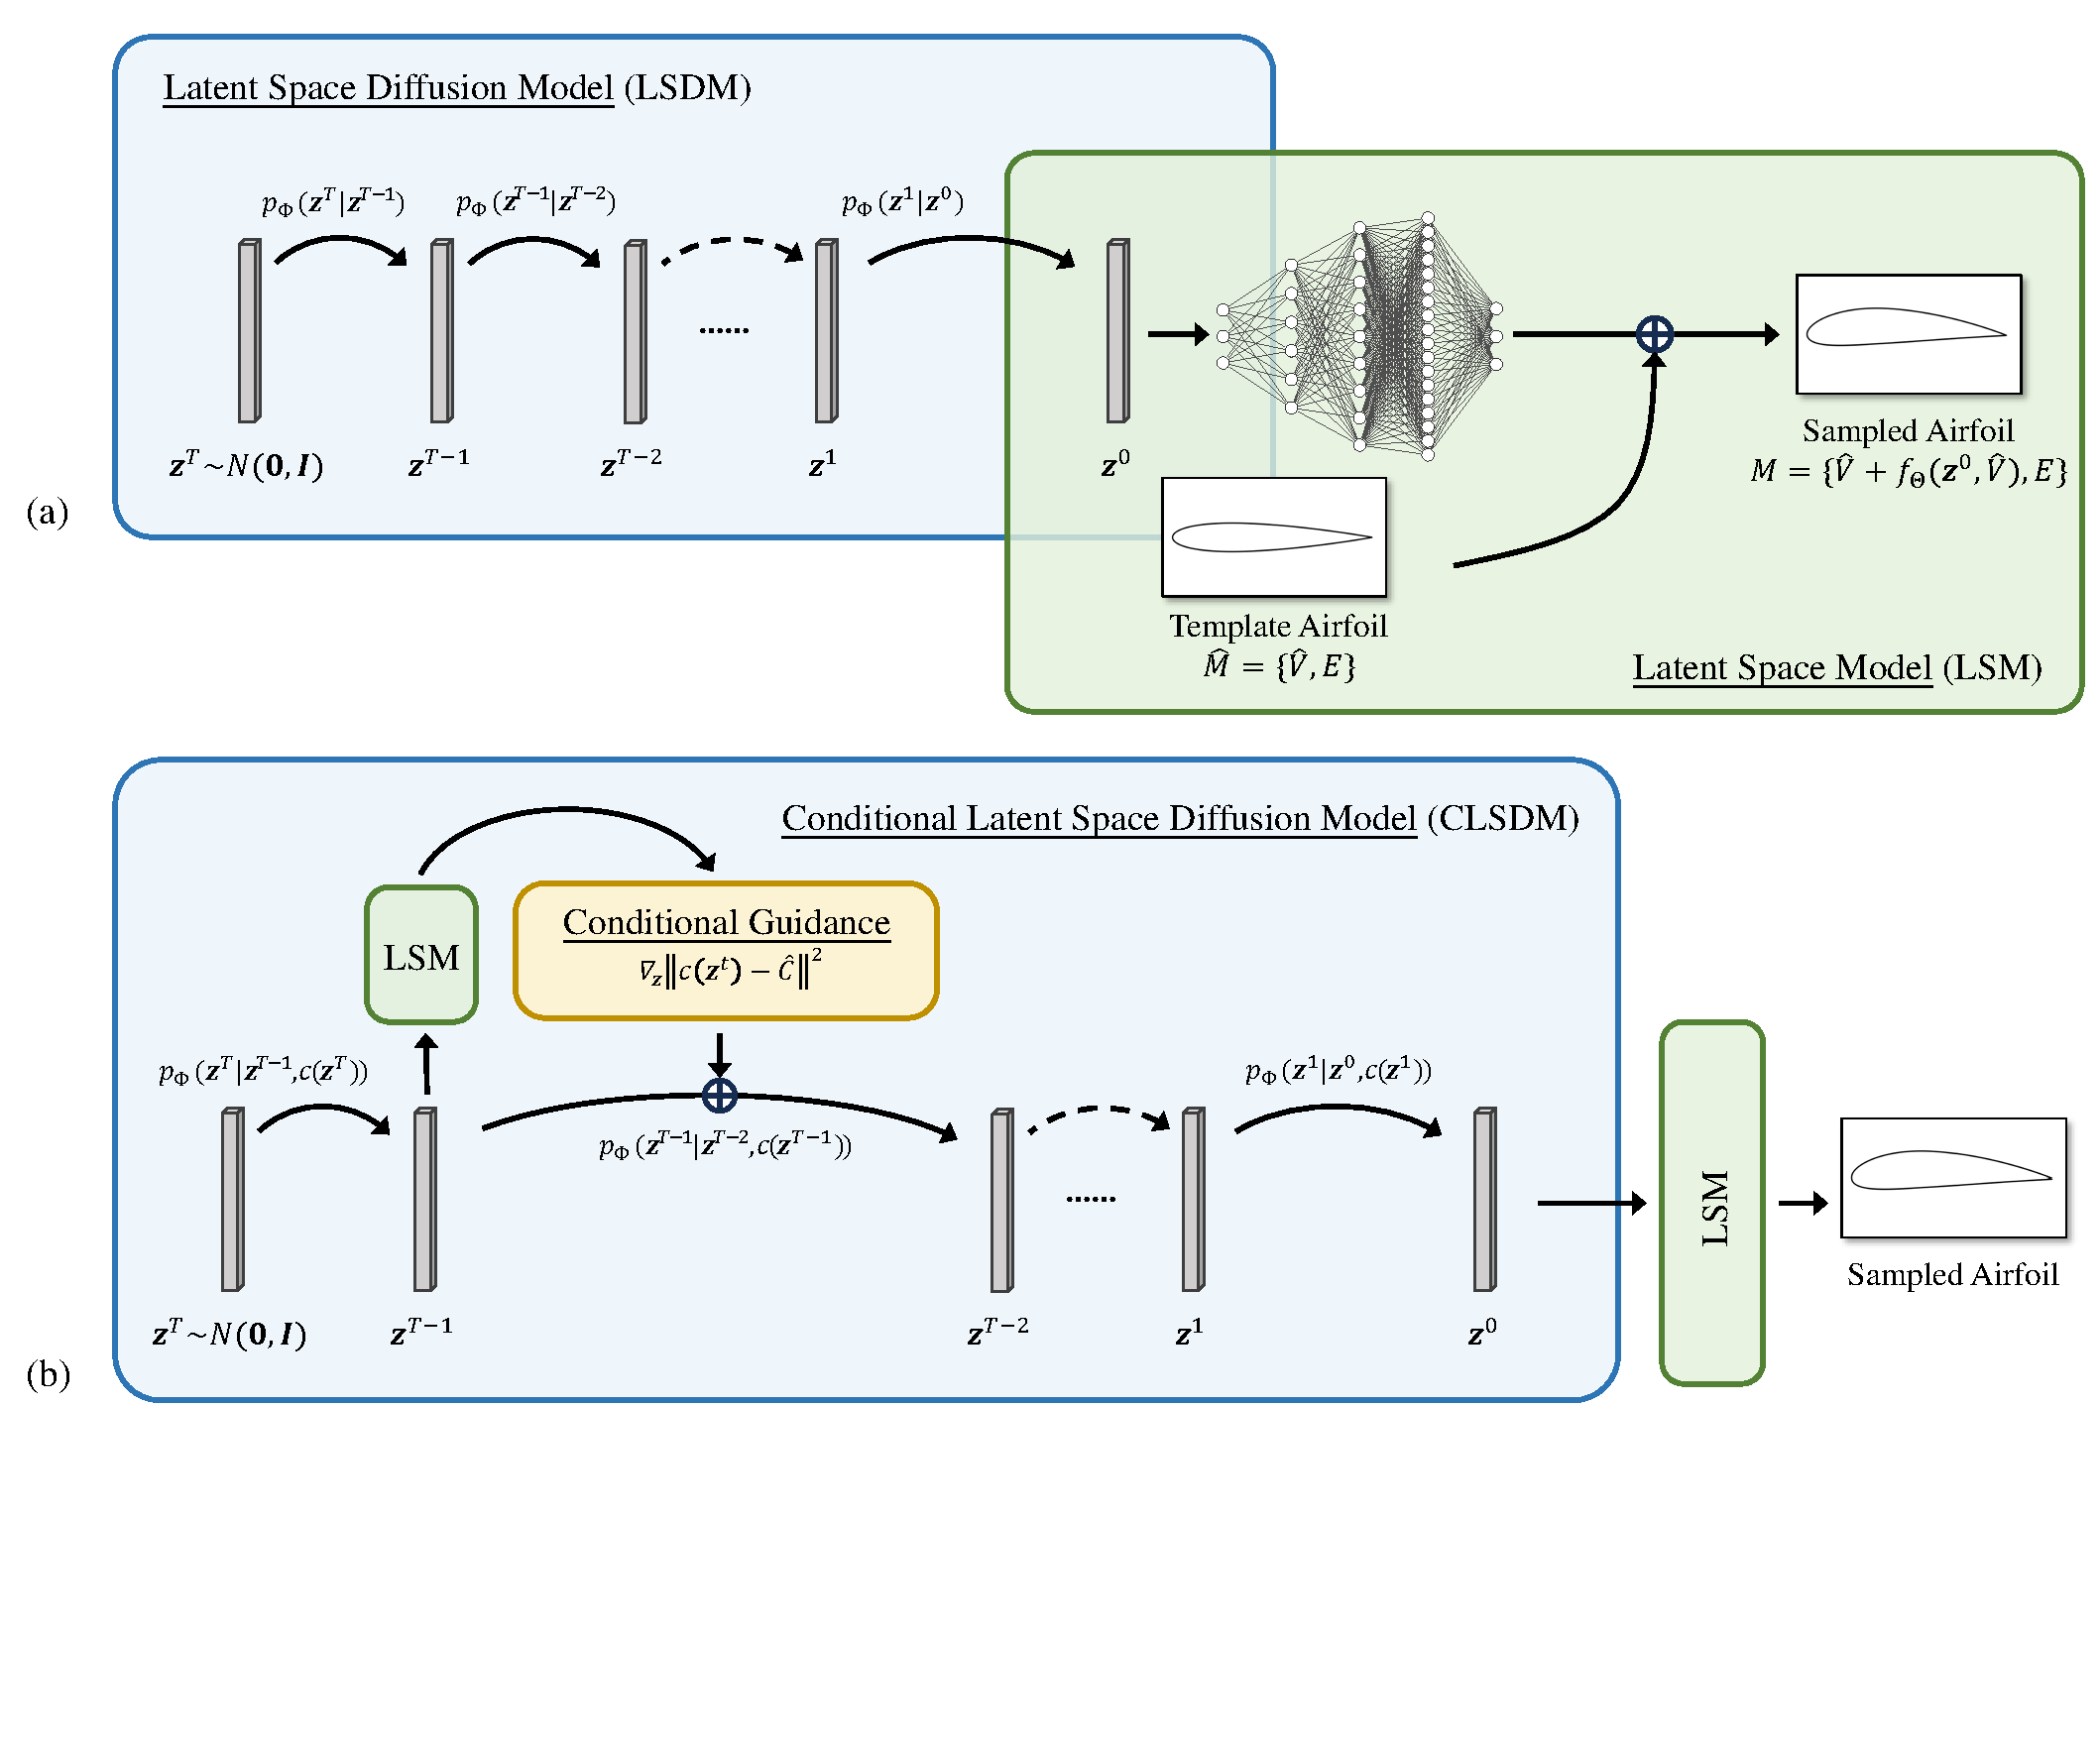
\includegraphics[width=1\linewidth]{chapter6/fig/framework.pdf}
    \end{center}
    \vspace{-4mm}
    \caption{
        \small \textit{DiffGeo} framework. (a) Unconditional \textit{DiffGeo} and (b) conditional \textit{DiffGeo}.
    }
    \label{ch6:fig:abs_framework}
\end{figure}

\section{Introduction}

Design Space Exploration (DSE) is the systematic process of sampling, evaluating, and selecting candidate designs across a high-dimensional geometry space to satisfy multiple objectives and constraints. In aerospace engineering, DSE constitutes a foundational step in aerodynamic shape optimization (ASO) and multidisciplinary design optimization (MDO) with many practical applications. Traditionally, DSE is implemented by combining low-dimensional, handcrafted parameterizations--such as Bézier curves, B-splines or Class/Shape Transformation (CST)~\cite{aa.Kulfan2008}--with statistical sampling techniques like Latin hypercube sampling (LHS)~\cite{ai.McKay1979} and surrogate modeling to approximate expensive performance evaluations. While effective, this paradigm can prove inefficient, inflexible and iterative for several reasons. First, traditional DSE workflows often requires dedicated shape modeling to ensure the generation of valid and related designs, including the choice of an appropriate shape parameterization and subsequent hyperparameter tuning. This process involves imposing extensive constraints on shape variables and managing the trade-off between design space exploration and exploitation. Second, these methods are usually restricted to low-dimensional design spaces, which limits their ability to capture complex geometric variations. Third, the usual reliance on Monte Carlo–style `sampling-evaluation-selection' often requires many random samples and performance evaluations to meet the design objectives, which is inefficient. This is because the sampling process is passive and cannot be actively guided toward feasible or high-performing regions of the design space. This lack of sampling control is particularly limiting when addressing complex, high-dimensional design objectives and constraints. This ultimately restricts the adaptability and effectiveness of the design process.

Recent advances in machine learning offer a promising way to overcome these limitations. Deep generative design methods train models to directly synthesize new designs by learning from prior examples through supervised, data-driven optimization. By capturing the joint distribution of feasible geometries, performance and constraints, these models can generate candidate designs that satisfy desired criteria in one shot. Early applications of deep generative models to aerodynamic design have demonstrated this potential. For example, conditional generative adversarial networks (GANs)~\cite{ai.Goodfellow2020} and variational autoencoders (VAEs)~\cite{ai.Kingma2015} have been used to generate 2D airfoils conditioned on target aerodynamic properties~\cite{aa.Chen2020,aa.Li2020,aa.Li2021,aa.Du2020,aa.Achour2020,aa.Wang2022,aa.Lei2021,aa.Yonekura2021,aa.Kou2023,aa.Swannet2024}. These studies have confirmed the feasibility of learning-based shape generation but also suffer from some limitations.  First, most models require large training datasets, often on the order of $10^3$ samples for 2D airfoils for example, to generate meaningful and diverse designs. Such data demands can rarely be met in aerospace engineering, where diverse and representative shapes are costly to obtained. Second, existing generative models entangle geometry with performance in a way that limits adaptability, particularly given the highly customized nature of design requirements. In other words, a model trained for a specific task, such as low-speed, lift-conditioned airfoil generation, cannot be easily repurposed for different scenarios or objectives without collecting new data and retraining. Third, controllability over the generated designs remains limited. Most models only accept a few scalar values, such as  body forces or operating conditions, as conditioning inputs, making it difficult to impose more complex constraints, such as spanwise thickness distributions or 3D geometry profiling. In summary, current data-driven generative DSE approaches require a significant amount of data, cannot adapt easily to new design objectives, and do not provide fine-grained and effective controllability for design space exploration.

To address these challenges, we introduce \textit{DiffGeo}, a novel deep generative method for DSE in multidisciplinary design optimization. An early version of this approach was presented in a conference paper~\cite{aa.Wei2024}. It focused on 2D airfoils and this paper generalizes it to a wider range of geometries and shows it can be turned into a widely applicable DSE tool. As shown in Fig.~\ref{ch6:fig:abs_framework}, \textit{DiffGeo} is built upon a diffusion-based generative model~\cite{ai.SohlDickstein2015} that operates on a shape latent space learned using an automated parameterization method~\cite{aa.Wei2023,aa.Wei2023b}. When guided by task-specific energy functions, \textit{DiffGeo} can efficiently generate aerodynamic geometries satisfying complex design objectives.  We show that diffusion-based sampling offers more stable training than  GAN- and VAE-based approaches,  eliminating the need for adversarial discriminators and enabling data-efficient model training. Crucially, \textit{DiffGeo} is designed to provide a task-agnostic shape sampler independent of any performance target. When applied to new tasks, it allows rapid adaptation by simply replacing or combining one or more differentiable energy functions as guidance, without having to retrain the whole model. Notably, we introduce an enhanced conditional generation scheme to further improve the controllability of complex guidance.

In short, we aim to establish \textit{DiffGeo} as a novel generative framework for design space exploration. Our key contributions include:
%
\begin{itemize}
    \item \textbf{High data efficiency.} \textit{DiffGeo} can be effectively trained in data-scarce environments to construct a meaningful design space and to enable its exploration. For example, our experiments show successful training with as few as 50 airfoils or 75 3D blades linearly interpolated from six base profiles, which is one to two orders of magnitude less data than prior deep generative models. This reduces the data requirements by one or two orders of magnitude, compared  to GAN- and VAE-based approaches. By drastically lowering the data barrier, \textit{DiffGeo} enables generative DSE when large-scale geometry databases cannot be obtained, which is often the case in aerospace engineering.

    \item \textbf{Geometry-performance disentanglement.} \textit{DiffGeo} decouples geometry generation from task-specific objectives, making the core shape generator general-purpose and reusable. When adapting to different tasks, new objectives and constraints are imposed via energy functions during sampling, without retraining the underlying generator.

    \item \textbf{Controllability Under High-Dimensional Constraints.} \textit{DiffGeo} supports fine-grained, multi-parameter conditioning giving designers precise control over the generated geometry with complex, vector-valued conditions, such as twisting distributions along a 3D rotor blade. This enables exploration of designs that satisfy spatially varying constraints, a capability absent in existing generative design tools.
\end{itemize}
%
Although we focus on geometric design objectives in this study, the framework could be extended to performance-based objectives and this will be the subject of future work. 

The remainder of this paper is structured as follows. Section~\ref{ch6:sec:related_work} discusses the context of related methods in design space exploration, including conventional design of experiments, data-driven model and generation-based approaches. Section~\ref{ch6:sec:method} describes \textit{DiffGeo}'s technical details. Section~\ref{ch6:sec:exp} evaluates \textit{DiffGeo} across three case studies: (i) a 2D airfoil generation benchmark that compares \textit{DiffGeo} with GAN- and VAE-based methods on sample quality, diversity, and controllability under extreme low-data conditions; (ii) task-informed data generation with \textit{DiffGeo} for improving surrogate-based optimization; and (iii) 3D turbomachinery blade prototyping with strict geometric constraints and limited reference designs. Finally, Section~\ref{ch6:sec:conclusion} concludes the paper, discusses \textit{DiffGeo}'s broader impact and proposes directions for future work.